\section{\sysname}
\label{SEC:architecture}

\cappos{this section is meant to describe the mechanisms / changes that were
made to docker to support \sysname.  So, one likely organization would be
to discuss each of the components (infrakit, swarmkit, notary) in some detail
while emphasizing the mechanisms that were added.  I've started the section
with an example to get it started}

There are three critical components that have been altered that enable
\sysname (Figure~XXX\cappos{need to add}).  First, infrakit is the component 
of Docker which handles container
instantiation and XXX on a local system.  Infrakit was modified by changing
YYY to enable ZZZ.   Swarmkit enables the instantatiation and management of 
groups of containers by XXX.  ...

\subsection{Infrakit}

\cappos{describe purpose and concepts about how this is designed.  Try to 
avoid talking too much about how it is actually used at this point.  To 
think of a car analogy, you don't want a user's manual here, you want the
mechanics guide / tech specs for making the components.}


\subsection{Swarmkit}
Swarmkit handles mutual TLS, ...


\subsection{Notary}
Notary enables key expiry, trust anchoring, etc...

\cappos{Content from:
\url{https://docs.docker.com/engine/security/trust/content_trust/}}



When transferring data among networked systems, trust is a central concern.
In particular, when communicating over an untrusted medium such as the
internet, it is critical to ensure the integrity and the publisher of all
the data a system operates on. You use Docker Engine to push and pull
images (data) to a public or private registry. Content trust gives you the
ability to verify both the integrity and the publisher of all the data
received from a registry over any channel.

\subsubsection{Understanding trust in Docker}
Content trust allows operations with a remote Docker registry to enforce
client-side signing and verification of image tags. Content trust provides
the ability to use digital signatures for data sent to and received from
remote Docker registries. These signatures allow client-side verification
of the integrity and publisher of specific image tags.

Currently, content trust is disabled by default. To enable it, set the
{\tt DOCKER\_CONTENT\_TRUST} environment variable to 1. Refer to the environment
variables and Notary configuration for the docker client for more options.

Once content trust is enabled, image publishers can sign their images.
Image consumers can ensure that the images they use are signed. Publishers
and consumers can be individuals alone or in organizations. Docker’s
content trust supports users and automated processes such as builds.

\subsubsection{Image tags and content trust}
An individual image record has the following identifier:

\begin{quote}
[REGISTRY\_HOST[:REGISTRY\_PORT]/]REPOSITORY[:TAG]
\end{quote}

A particular image REPOSITORY can have multiple tags. For example, latest
and 3.1.2 are both tags on the mongo image. An image publisher can build an
image and tag combination many times changing the image with each build.

Content trust is associated with the TAG portion of an image. Each image
repository has a set of keys that image publishers use to sign an image
tag. Image publishers have discretion on which tags they sign.

An image repository can contain an image with one tag that is signed and
another tag that is not (Figure~\ref{fig-notary-tag-signing}). For example, 
consider the Mongo image repository.
The latest tag could be unsigned while the 3.1.6 tag could be signed. It is
the responsibility of the image publisher to decide if an image tag is
signed or not. In this representation, some image tags are signed, others
are not:

\begin{figure}[t]
  \center{}
  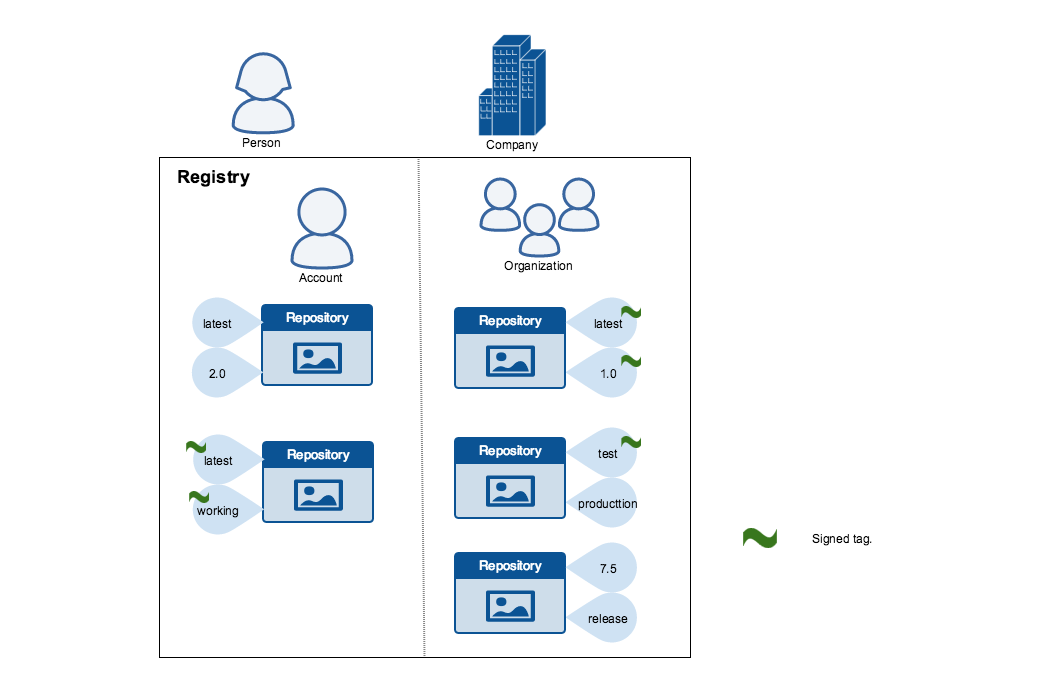
\includegraphics[width=.5\textwidth]{images/notary_tag_signing.png}
  \caption{Tag signing in Notary.
  \label{fig-notary-tag-signing} }
\end{figure}

Publishers can choose to sign a specific tag or not. As a result, the
content of an unsigned tag and that of a signed tag with the same name may
not match. For example, a publisher can push a tagged image
someimage:latest and sign it. Later, the same publisher can push an
unsigned someimage:latest image. This second push replaces the last
unsigned tag latest but does not affect the signed latest version. The
ability to choose which tags they can sign, allows publishers to iterate
over the unsigned version of an image before officially signing it.

Image consumers can enable content trust to ensure that images they use
were signed. If a consumer enables content trust, they can only pull, run,
or build with trusted images. Enabling content trust is like wearing a pair
of rose-colored glasses. Consumers “see” only signed image tags and the
less desirable, unsigned image tags are “invisible” to them.

\begin{figure}[t]
  \center{}
  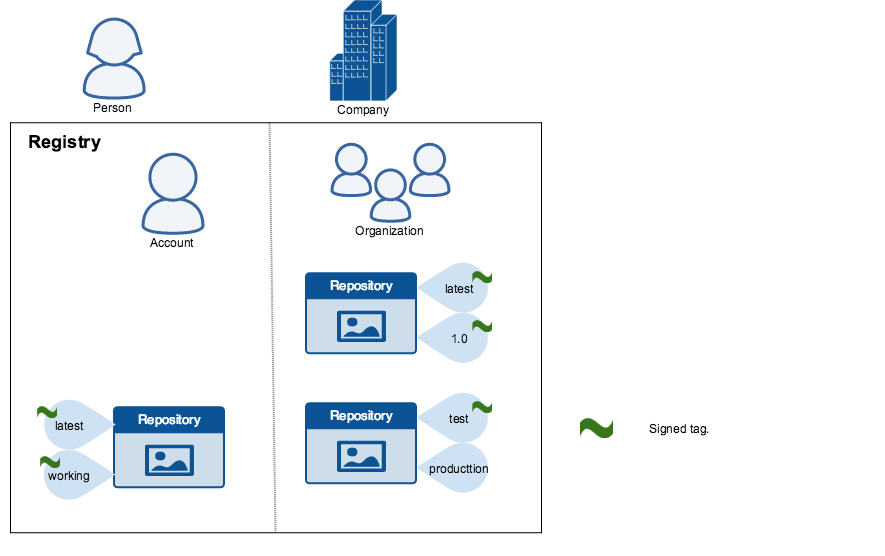
\includegraphics[width=.5\textwidth]{images/notary_trust_view.png}
  \caption{
This figure depicts the various signing keys and their
relationships.  \cappos{Where is this figure used in the text?}
  \label{fig-notary-trust-view} }
\end{figure}

To the consumer who has not enabled content trust, nothing about how they
work with Docker images changes. Every image is visible regardless of
whether it is signed or not.

\subsubsection{Content trust operations and keys}
When content trust is enabled, docker CLI commands that operate on tagged
images must either have content signatures or explicit content hashes. The
commands that operate with content trust are:

push
build
create
pull
run
For example, with content trust enabled a docker pull someimage:latest only
succeeds if someimage:latest is signed. However, an operation with an
explicit content hash always succeeds as long as the hash exists:

\begin{quote}
\$ docker pull
someimage@sha256:d149ab53f8718e987c3a3024bb8aa0e2caadf6c0328f1d9d850b2a2a67f2819a
\end{quote}

Trust for an image tag is managed through the use of signing keys. A key
set is created when an operation using content trust is first invoked. A
key set consists of the following classes of keys:

\begin{itemize}
\item an offline key that is the root of content trust for an image tag
repository or tagging keys that sign tags
\item server-managed keys such as the timestamp key, which provides freshness
security guarantees for your repository
\end{itemize}

\begin{figure}[t]
  \center{}
  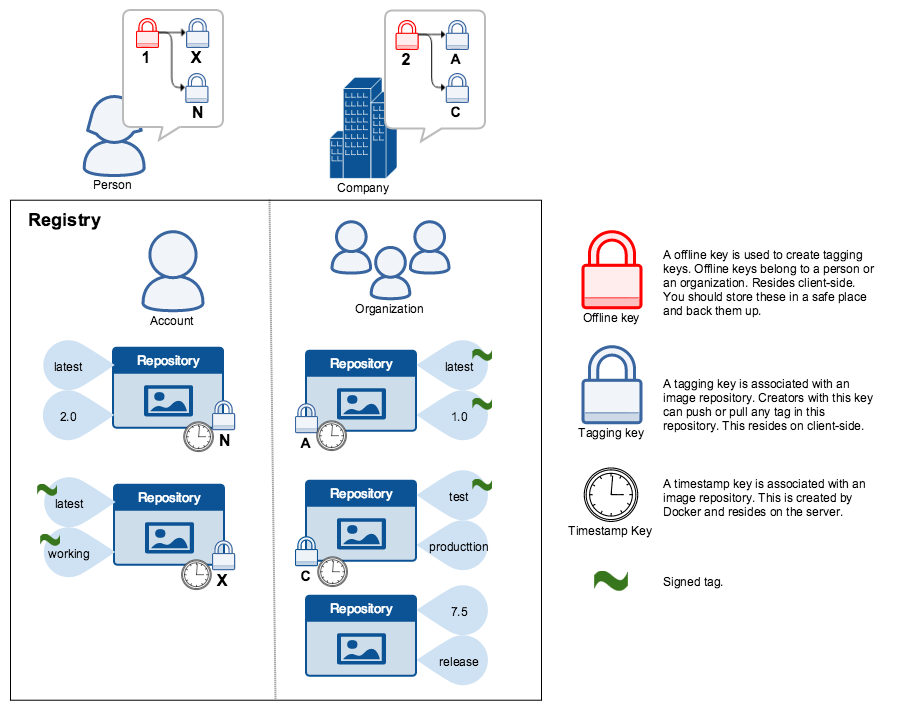
\includegraphics[width=.5\textwidth]{images/notary_trust_components.png}
  \caption{
This figure depicts the various signing keys and their
relationships.
  \label{fig-notary-components} }
\end{figure}

WARNING: Loss of the root key is very difficult to recover from. Correcting
this loss requires intervention from Docker Support to reset the repository
state. This loss also requires manual intervention from every consumer that
used a signed tag from this repository prior to the loss.
You should backup the root key somewhere safe. Given that it is only
required to create new repositories, it is a good idea to store it offline
in hardware. For details on securing, and backing up your keys, make sure
you read how to manage keys for content trust.

\subsubsection{Survey of typical content trust operations}
This section surveys the typical trusted operations users perform with
Docker images. Specifically, we will be going through the following steps
to help us exercise these various trusted operations:

Build and push an unsigned image
Pull an unsigned image
Build and push a signed image
Pull the signed image pushed above
Pull unsigned image pushed above
Enable and disable content trust per-shell or per-invocation
In a shell, you can enable content trust by setting the
{\tt DOCKER\_CONTENT\_TRUST} environment variable. Enabling per-shell is useful
because you can have one shell configured for trusted operations and
another terminal shell for untrusted operations. You can also add this
declaration to your shell profile to have it turned on always by default.

To enable content trust in a bash shell enter the following command:

\begin{quote}
export DOCKER\_CONTENT\_TRUST=1
\end{quote}

Once set, each of the “tag” operations requires a key for a trusted tag.

In an environment where {\tt DOCKER\_CONTENT\_TRUST} is set, you can use the
--disable-content-trust flag to run individual operations on tagged images
without content trust on an as-needed basis.

Consider the following Dockerfile that uses an untrusted base image:

\begin{quote}
\$  cat Dockerfile
FROM docker/trusttest:latest
RUN echo
\end{quote}

In order to build a container successfully using this Dockerfile, one can
do:

\begin{quote}
\$  docker build --disable-content-trust -t <username>/nottrusttest:latest .
Sending build context to Docker daemon 42.84 MB
...
Successfully built f21b872447dc
\end{quote}

The same is true for all the other commands, such as pull and push:

\begin{quote}
\$  docker pull --disable-content-trust docker/trusttest:latest
...
\$  docker push --disable-content-trust <username>/nottrusttest:latest
...
\end{quote}

To invoke a command with content trust enabled regardless of whether or how
the {\tt DOCKER\_CONTENT\_TRUST} variable is set:

\begin{quote}
\$  docker build --disable-content-trust=false -t
<username>/trusttest:testing .
\end{quote}

All of the trusted operations support the --disable-content-trust flag.

\subsubsection{Push trusted content}
To create signed content for a specific image tag, simply enable content
trust and push a tagged image. If this is the first time you have pushed an
image using content trust on your system, the session looks like this:

\begin{quote}
\$ docker push <username>/trusttest:testing
The push refers to a repository [docker.io/<username>/trusttest] (len: 1)
9a61b6b1315e: Image already exists
902b87aaaec9: Image already exists
latest: digest:
sha256:d02adacee0ac7a5be140adb94fa1dae64f4e71a68696e7f8e7cbf9db8dd49418
size: 3220
Signing and pushing trust metadata
You are about to create a new root signing key passphrase. This passphrase
will be used to protect the most sensitive key in your signing system.
Please
choose a long, complex passphrase and be careful to keep the password and
the
key file itself secure and backed up. It is highly recommended that you use
a
password manager to generate the passphrase and keep it safe. There will be
no
way to recover this key. You can find the key in your config directory.
Enter passphrase for new root key with id a1d96fb:
Repeat passphrase for new root key with id a1d96fb:
Enter passphrase for new repository key with id
docker.io/<username>/trusttest (3a932f1):
Repeat passphrase for new repository key with id
docker.io/<username>/trusttest (3a932f1):
Finished initializing "docker.io/<username>/trusttest"
\end{quote}

When you push your first tagged image with content trust enabled, the
docker client recognizes this is your first push and:

alerts you that it will create a new root key
requests a passphrase for the root key
generates a root key in the ~/.docker/trust directory
requests a passphrase for the repository key
generates a repository key in the ~/.docker/trust directory
The passphrase you chose for both the root key and your repository key-pair
should be randomly generated and stored in a password manager.

NOTE: If you omit the testing tag, content trust is skipped. This is true
even if content trust is enabled and even if this is your first push.
\begin{quote}
\$ docker push <username>/trusttest
The push refers to a repository [docker.io/<username>/trusttest] (len: 1)
9a61b6b1315e: Image successfully pushed
902b87aaaec9: Image successfully pushed
latest: digest:
sha256:a9a9c4402604b703bed1c847f6d85faac97686e48c579bd9c3b0fa6694a398fc
size: 3220
No tag specified, skipping trust metadata push
\end{quote}

It is skipped because as the message states, you did not supply an image
TAG value. In Docker content trust, signatures are associated with tags.

Once you have a root key on your system, subsequent images repositories you
create can use that same root key:

\begin{quote}
\$ docker push docker.io/<username>/otherimage:latest
The push refers to a repository [docker.io/<username>/otherimage] (len: 1)
a9539b34a6ab: Image successfully pushed
b3dbab3810fc: Image successfully pushed
latest: digest:
sha256:d2ba1e603661a59940bfad7072eba698b79a8b20ccbb4e3bfb6f9e367ea43939
size: 3346
Signing and pushing trust metadata
Enter key passphrase for root key with id a1d96fb:
Enter passphrase for new repository key with id
docker.io/<username>/otherimage (bb045e3):
Repeat passphrase for new repository key with id
docker.io/<username>/otherimage (bb045e3):
Finished initializing "docker.io/<username>/otherimage"
\end{quote}

The new image has its own repository key and timestamp key. The latest tag
is signed with both of these.

\subsubsection{Pull image content}
A common way to consume an image is to pull it. With content trust enabled,
the Docker client only allows docker pull to retrieve signed images. Let’s
try to pull the image you signed and pushed earlier:

\begin{quote}
\$  docker pull <username>/trusttest:testing
Pull (1 of 1): <username>/trusttest:testing@sha256:d149ab53f871
...
Tagging <username>/trusttest@sha256:d149ab53f871 as
docker/trusttest:testing
\end{quote}

In the following example, the command does not specify a tag, so the system
uses the latest tag by default again and the docker/trusttest:latest tag is
not signed.

\begin{quote}
\$ docker pull docker/trusttest
Using default tag: latest
no trust data available
\end{quote}

Because the tag docker/trusttest:latest is not trusted, the pull fails.

\cappos{the notary text was too much like running examples.  It needs to focus
on the design at a higher level.}
